% % % % % % % % % % % % % % % % % % % % % % % % % % % % % % % % % %
\documentclass[runningheads]{llncs}

% packages
\usepackage{xspace}
\usepackage{ifthen}
\usepackage{amsbsy}
\usepackage{amssymb}
\usepackage{balance}
\usepackage{booktabs}
\usepackage{graphicx}
\usepackage{multirow}
\usepackage{needspace}
\usepackage{microtype}
\usepackage{bold-extra}

% constants
\newcommand{\Title}{Aspect-based refactoring}
\newcommand{\TitleShort}{\Title}
\newcommand{\Authors}{Santiago Vidal, Claudia Marcos, Alexandre Bergel, Gabriela Ar\'evalo}
\newcommand{\AuthorsShort}{S. Vidal, C. Marcos, A. Bergel, G. Ar\'evalo}

% references
\usepackage[colorlinks]{hyperref}
\usepackage[all]{hypcap}
\setcounter{tocdepth}{2}
\hypersetup{
	colorlinks=true,
	urlcolor=black,
	linkcolor=black,
	citecolor=black,
	plainpages=false,
	bookmarksopen=true,
	pdfauthor={\Authors},
	pdftitle={\Title}}

\def\chapterautorefname{Chapter}
\def\appendixautorefname{Appendix}
\def\sectionautorefname{Section}
\def\subsectionautorefname{Section}
\def\figureautorefname{Figure}
\def\tableautorefname{Table}
\def\listingautorefname{Listing}

% source code
\usepackage{xcolor}
\usepackage{textcomp}
\usepackage{listings}
\definecolor{source}{gray}{0.9}
\lstset{
	language={},
	% characters
	tabsize=3,
	upquote=true,
	escapechar={!},
	keepspaces=true,
	breaklines=true,
	alsoletter={\#:},
	breakautoindent=true,
	columns=fullflexible,
	showstringspaces=false,
	basicstyle=\footnotesize\ttfamily,
	% background
	frame=single,
    framerule=0pt,
	backgroundcolor=\color{source},
	% numbering
	numbersep=5pt,
	numberstyle=\tiny,
	numberfirstline=true,
	% captioning
	captionpos=b,
	% formatting (html)
	moredelim=[is][\textbf]{<b>}{</b>},
	moredelim=[is][\textit]{<i>}{</i>},
	moredelim=[is][\color{red}\uwave]{<u>}{</u>},
	moredelim=[is][\color{red}\sout]{<del>}{</del>},
	moredelim=[is][\color{blue}\underline]{<ins>}{</ins>}}
\newcommand{\ct}{\lstinline[backgroundcolor=\color{white},basicstyle=\footnotesize\ttfamily]}
\newcommand{\lct}[1]{{\small\tt #1}}

% tikz
% \usepackage{tikz}
% \usetikzlibrary{matrix}
% \usetikzlibrary{arrows}
% \usetikzlibrary{external}
% \usetikzlibrary{positioning}
% \usetikzlibrary{shapes.multipart}
% 
% \tikzset{
% 	every picture/.style={semithick},
% 	every text node part/.style={align=center}}
% \tikzexternalize[prefix=figures/]{quality}

% proof-reading
\usepackage{xcolor}
\usepackage[normalem]{ulem}
\newcommand{\ra}{$\rightarrow$}
\newcommand{\ugh}[1]{\textcolor{red}{\uwave{#1}}} % please rephrase
\newcommand{\ins}[1]{\textcolor{blue}{\uline{#1}}} % please insert
\newcommand{\del}[1]{\textcolor{red}{\sout{#1}}} % please delete
\newcommand{\chg}[2]{\textcolor{red}{\sout{#1}}{\ra}\textcolor{blue}{\uline{#2}}} % please change
\newcommand{\chk}[1]{\textcolor{ForestGreen}{#1}} % changed, please check

% comments \nb{label}{color}{text}
\newboolean{showcomments}
\setboolean{showcomments}{true}
\ifthenelse{\boolean{showcomments}}
	{\newcommand{\nb}[3]{
		{\colorbox{#2}{\bfseries\sffamily\scriptsize\textcolor{white}{#1}}}
		{\textcolor{#2}{\sf\small$\blacktriangleright$\textit{#3}$\blacktriangleleft$}}}
	 \newcommand{\version}{\emph{\scriptsize$-$Id$-$}}}
	{\newcommand{\nb}[2]{}
	 \newcommand{\version}{}}
\newcommand{\rev}[2]{\nb{Reviewer #1}{red}{#2}}
\newcommand{\ab}[1]{\nb{Alexandre}{blue}{#1}}
\newcommand{\lr}[1]{\nb{Lukas}{orange}{#1}}

% graphics: \fig{position}{percentage-width}{filename}{caption}
\DeclareGraphicsExtensions{.png,.jpg,.pdf,.eps,.gif}
\graphicspath{{figures/}}
\newcommand{\fig}[4]{
	\begin{figure}[#1]
		\centering
		\includegraphics[width=#2\textwidth]{#3}
		\caption{\label{fig:#3}#4}
	\end{figure}}

% abbreviations
\newcommand{\ie}{\emph{i.e.,}\xspace}
\newcommand{\eg}{\emph{e.g.,}\xspace}
\newcommand{\etc}{\emph{etc.}\xspace}
\newcommand{\etal}{\emph{et al.}\xspace}

% lists
\newenvironment{bullets}[0]
	{\begin{itemize}}
	{\end{itemize}}

\newcommand{\seclabel}[1]{\label{sec:#1}}
\newcommand{\secref}[1]{Section~\ref{sec:#1}\xspace}

% D O C U M E N T
% % % % % % % % % % % % % % % % % % % % % % % % % % % % % % % % % %
\begin{document}

% T I T L E
% % % % % % % % % % % % % % % % % % % % % % % % % % % % % % % % % %

\title{\Title}
\titlerunning{\TitleShort}

\author{\Authors} 
\authorrunning{\AuthorsShort}

\institute{ISISTAN Research Institute, Faculty of Sciences,\\
 UNICEN University, Campus Universitario, Tandil, Buenos Aires,
Argentina\\
Also CONICET\\
Also CIC\\
PLEIAD Lab, Department of Computer Science (DCC),\\
	University of Chile, Santiago, Chile,
...}

\maketitle

% A B S T R A C T
% % % % % % % % % % % % % % % % % % % % % % % % % % % % % % % % % %

\begin{abstract}
an abstract
\end{abstract}

% % % % % % % % % % % % % % % % % % % % % % % % % % % % % % % % % %
\section{Introduction}\seclabel{introduction}

The story to tell in this paper is the following one:
1) We have the actual Mondrian code
2) Santiago have extracted the CC into pragmas
3) He has identified different possible pragmas. Here some patterns could be identified based on the code (That's the POINT of the paper)
4) Once we have the pragmas, we can think of an injection machine to produce new code.
This new code is semantically equivalent to the original one, but not syntactically the same. This is not so important since all the large set of Mondrian unit tests has the last word on it.

Then the core of the paper will be the Different patterns of hand written code that are rewritten (refactored?) with pragmas 

justificar el xq se quiere refactorizar los cache 

\ab{what is the link with your previous work? Is there some hypothesis that you validate with the experiment on Mondrian?}

\ab{this is just a try, we will probably refine that later} This work presented in this paper makes the following contributions:
\begin{itemize}
\item Identification and composition of pattern for memoization techniques
\item Associating code quality metrics and AOP-based refactoring. \ab{refactoring Mondrian increases its quality (we can use macCabe complexity, number of lines of code, number of methods, ...)}
\item General technique of implementing memoization with AOP
\end{itemize}

% % % % % % % % % % % % % % % % % % % % % % % % % % % % % % % % % %
\section{Modularly defining caches in Mondrian}\seclabel{problem}

\paragraph{Context.} Mondrian\footnote{\url{http://www.moosetechnology.org/tools/mondrian}}~\cite{Meye06a} is an open and agile visualization library. 
Mondrian uses a graph, made of possibly nested nodes and edges, to describe a visualization. Mondrian is a crucial component which is used in more than a dozen of independent projects. To meet clients performance requirements, Mondrian's authors are paying a great attention to provide fast and scalable rendering. To that purpose, Mondrian contains a number of cache mechanisms to avoid redundant code executions. These caches were introduced gradually, according to emerging requirements.

Mondrian is now on the verge to become a visualization engine framework versus a library as it is currently. Mondrian is now used in situations that were not originally planned. For example, Mondrian has been used to visualize the behavior of animated robots, whereas Mondrian has been originally designed to visualize software source code~\cite{Lanz03d}. The caches that are intensively used when visualizing software are not useful and may even be a source of slowdown and complexity when visualizing animated robots. 

The future Mondrian framework must offer the possibility of selectively using and combining caches.

\paragraph{Problem.}

Modularizing caches cannot be realizing without loosing performances.
Currently, the caches are implemented by means of a dedicated variable
that is defined in the MOGraphElement class. That is to say, for each
new cache that is added, a variable must be defined. The basic functionalities
of the caches are store/get a value and reset. So, if the goal of
the refactorization is the extraction of the \emph{Cache Concern}
by means of the creation of a specific class to delegate the behavior
of the caches, it must have these functionalities. For example, could
be used a strategy which uses a class containing a collection of caches
and each cache can contain different types of items (as is shown in
Fig. \ref{fig:Cache-behaviour-delegation.}). In this case, all the
cache variables and the fragments of code of the methods in which
they were used were encapsulated using the \emph{Cache} class and
creating a suitable \emph{CacheableItem}. In \emph{MOGraphElement}
hierarchy only remain a reference to the \emph{Cache} class that contains
all the caches. However, this kind of modularization looses performances
because the access to the cache variable is not direct. This causes
a delay when attempting to access the values that keep the caches.
So, the separation of this concern is not a trivial problem. Specifically,
when this solution the caches mechanism was 3 to 10 times slower,
being the delay proportional to the number of elements.

%
\begin{figure}
\begin{centering}
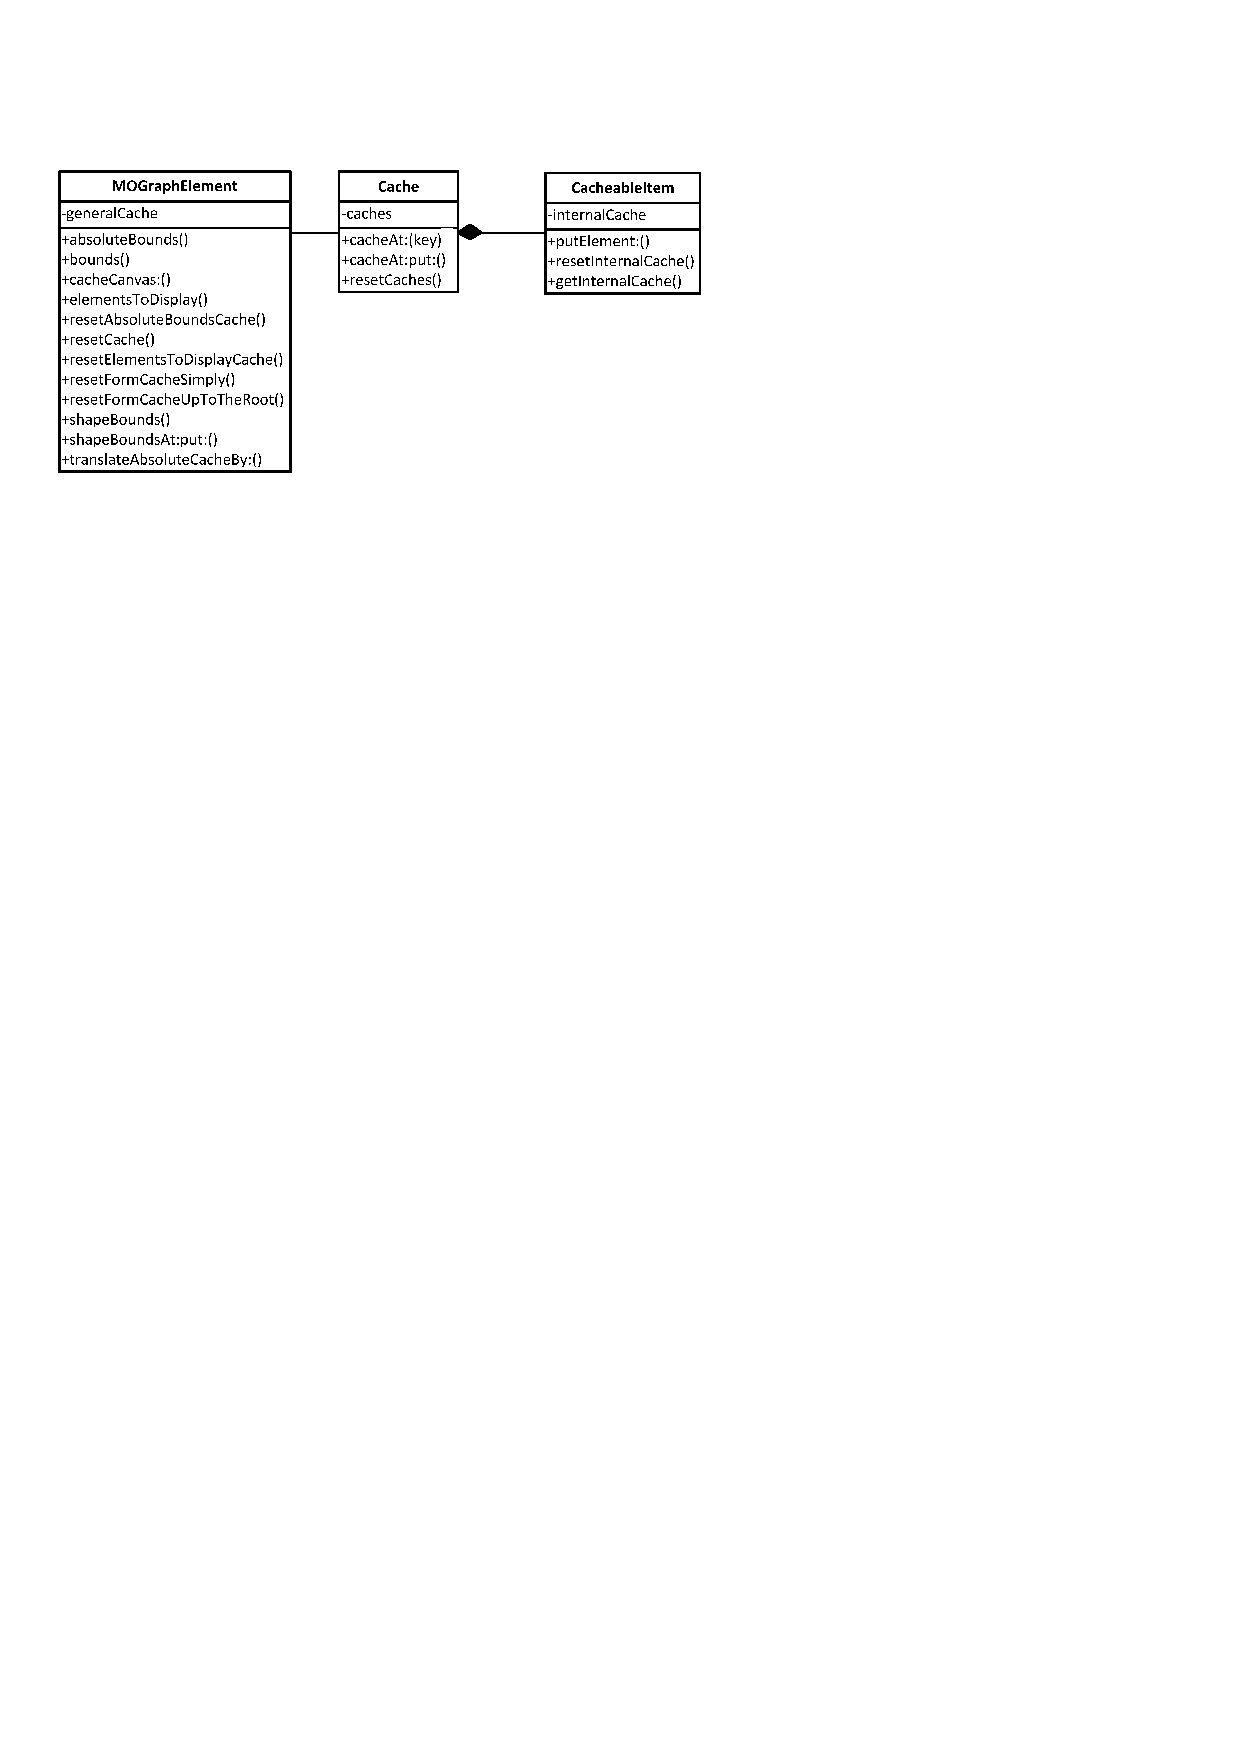
\includegraphics{CacheMechanisms} 
\par\end{centering}

\caption{Cache behavior delegation.\label{fig:Cache-behaviour-delegation.}}

\end{figure}

% % % % % % % % % % % % % % % % % % % % % % % % % % % % % % % % % %
\section{Refactoring}\seclabel{refactoring}


The goal of the refactorization is the separation of the \emph{Cache
Concern} from the main class of \emph{Mondrian}: \emph{MOGraphElement}
and its subclasses (\emph{MOEdge}, \emph{MONode}, and \emph{MORoot}).
The refactoring process begins with the identification of the caches.
This initial identification of the caches is done with the information
provided by the developers of Mondrian and it lies in to know the
variables related to the caches and the places where they are used.
Nine different caches are found in Mondrian: \emph{cacheShapeBounds},
\emph{cacheForm}, \emph{boundsCache}, \emph{absoluteBoundsCache},
\emph{elementsToDisplayCache}, \emph{lookupNodeCache}, \emph{cacheFromPoint},
\emph{cacheToPoint}, and \emph{cacheBounds}. Each of them has a different
internal structure according on what is stored. After this initial
identification, the fragment of codes in which the caches are used
are grouped together based on the purpose of its use. As mentioned
in the previous section, the main general purposes identified are: 
\begin{itemize}
\item Initialize and reset the cache. 
\item Get the data stored in the cache. 
\item Store data in the cache. 
\end{itemize}
The task of group the fragments of code of the different caches is
achieved with the goal of identifying possible strategies for refactoring.
In this line, some subgroups of similar functionalities are found.
These subgroups allows the identification of code patterns that are
repeated in the use of the caches. Once the patterns are identified,
a refactoring strategy is applied. These steps are described in the
following subsections.


\subsection{Pattern Description\label{sub:Pattern-Identification}}

In this section, the main code patterns that we identified are presented.
Each pattern is described with the most relevant typical occurrence,
the number of occurrences of the pattern and a code example. The purpose
of the code examples is to illustrate the occurrences of each pattern
in the proper context.

\emph{Reset Cache}: this pattern represents a situation in which a
cache is reset. The reset structure is \emph{cache:=resetValue} where
\emph{resetValue} depends on the cache internal structure. Typically,
the \emph{resetValue} is nil or a new of a kind of Dictionary object.
Eighteen occurrences of this pattern are found in the Mondrian code.
Next, the method \emph{resetCache} is presented as an example. In
this method the \emph{Reset Cache} pattern is repeated in four occasions
to reset the caches \emph{boundsCache}, \emph{absoluteBoundsCache},
\emph{cacheShapeBounds}, and \emph{elementsToDisplayCache}.

\begin{lstlisting} 
MOGraphElement>>resetCache 
	self resetElementsToLookup.
	boundsCache := nil. 
	absoluteBoundsCache := nil. 
	cacheShapeBounds :=SmallDictionary new. 
	elementsToDisplayCache := nil. 
	self resetMetricCaches
\end{lstlisting}

\emph{Return Cache with Precondition Checking}: this pattern shows
the situation in which a verification is accomplished before access
to a cache with the goal of avoid possible exceptions when the cache
is nil. Typically, the structure of this pattern is: \emph{if (cache==nil)
cache:=newValue. return cache}. Five occurrences of this pattern are
found in the Mondrian code. Next, the method \emph{bounds} is presented
as an example in which boundsCache is accessed.

\begin{lstlisting} 
MOEdge>>bounds  
	^ boundsCache ifNil:[boundsCache:= self shape computeBoundsFor: self ]. 
\end{lstlisting}

\emph{Cache Initialization}: this pattern represents a situation in
which a value is assigned to a cache. The structure of the pattern
is only an assignation: cache:=\emph{aValue}. This pattern is found
in three occasions. Next, the method \emph{cacheCanvas} is presented
as an example in which a value is assigned to cacheForm.

\begin{lstlisting} 
MOGraphElement>>cacheCanvas: aCanvas 
	cacheForm:= aCanvas form copy: ((self bounds origin + aCanvas origin 
	- (1@1)) extent: (self bounds extent + (2@2))). 
\end{lstlisting}

\emph{Return Cache}: this pattern shows the situation in which a cache
is accessed. The structure of the pattern is the return of the cache:
\emph{return cache}. This pattern is found in four occasions. Next,
the method \emph{shapeBounds} is presented as an example in which
cacheShapeBounds is accessed.

\begin{lstlisting} 
MOGraphElement>>shapeBounds  
	^ cacheShapeBounds
\end{lstlisting}

\emph{Cache Loaded}: this pattern check is a cache or a group of them
are loaded or conversely, if they are nil. So, the structure of the
pattern for a single cache is \emph{cache != nil}. This pattern is
found in two occasions. Next the method \emph{isCacheLoaded} is presented
as an example of this pattern.

\begin{lstlisting} 
MOGraphElement>>isCacheLoaded 
	^cacheForm notNil. 
\end{lstlisting}

Fig. \ref{fig:Pattern-locations-in} shows in which methods the patterns
were found.%
\begin{figure}
\begin{centering}
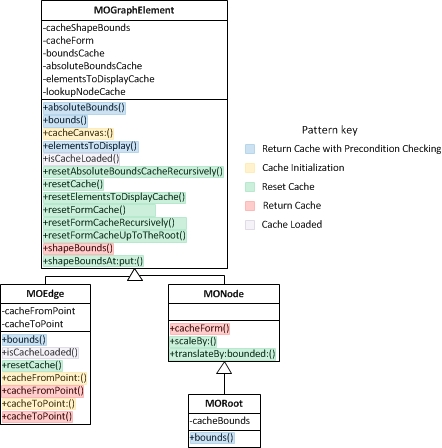
\includegraphics[scale=0.9]{PatternLocation} 
\par\end{centering}

\caption{Pattern locations in MOGraphElement hierarchy.\label{fig:Pattern-locations-in}}

\end{figure}


Additionally, Table \ref{tab:Cache-Concern-scattering} presents a
summary of the occurrences of each pattern in the MOGraphElement hierarchy,
the methods involved in each pattern, and the caches related with
a pattern.

%
\begin{table}
\begin{centering}
\begin{tabular}{|p{2.5cm}|c|c|p{3.5cm}|}
\hline 
Cache  & Occurrences  & Methods involved  & Caches involved\tabularnewline
\hline
\hline 
\emph{Reset Cache}  & 18 & 10 & boundsCache, absoluteBoundsCache, cacheShapeBounds, elementsToDisplayCache,
cacheForm, cacheFromPoint, cacheToPoint\tabularnewline
\hline 
\emph{Return Cache with Precondition Checking}  & 5 & 5 & elementsToDisplayCache, absoluteBoundsCache, boundsCache, cacheBounds\tabularnewline
\hline 
\emph{Cache Initialization}  & 3 & 3 & cacheForm, cacheFromPoint, cacheToPoint\tabularnewline
\hline 
\emph{Return Cache}  & 4 & 4 & cacheShapeBounds, cacheForm, cacheFromPoint, cacheToPoint\tabularnewline
\hline 
\emph{Cache Loaded} & 2 & 2 & cacheForm, cacheFromPoint, cacheToPoint\tabularnewline
\hline 
Total  & 32 & 24 & \multicolumn{1}{c}{}\tabularnewline
\cline{1-3} 
\end{tabular}
\par\end{centering}

\caption{Cache Concern scattering summary.\label{tab:Cache-Concern-scattering}}

\end{table}



\subsection{Refactoring Strategy}

Once the code patterns are identified, strategies to refactor them
are established. The main constraint to refactoring the code is the
preservation of a good performance of the cache mechanism.

Several alternatives were explored to encapsulated the \emph{Cache
Concern}. For example, one of the explored mechanisms was the separation
of the concern by means of the definition of an exclusive class for
managing caches. While this solution provided a good modular design,
it introduced indirections to access to the caches (\secref{problem}).
Indirections caused a poor performance that slows down response times
of the cache mechanism. For this reason, this is not a feasible solution.

After exploring a variety of options such as the use of proxies to
intercept messages, an approach based on code injection was chosen.
This solution has the advantage of encapsulating the concern in a
new unit while the code that it is finally executed after the injection
is similar to the original code of \emph{Mondrian}. So, the performance
is not affected. In order to encapsulate the source code related with
the code patterns the \emph{pragma} mechanism is used. \emph{Pragmas}
are the method annotation syntax implemented by Pharo.

The refactoring strategy used is: for each method that contained code
related to the \emph{Cache Concern}, the code related to the concern
is extracted using a pragma that is defined in the method. The decision
to define the pragma inside the method is in order to allow a better
visibility of the code that is injected. The pragmas used have a structure
according to each code pattern.\emph{ }In general, the pragmas structure
is \emph{$<$patternCodeName: cacheName$>$} where \emph{cacheName}
indicates the name of the cache that will be injected and \emph{patternCodeName}
indicates the pattern code to be generated. For example, the pragma
\emph{$<$ReturnCachePatternForCache: \#cacheShapeBounds$>$} indicates
that the \emph{Return Cache} pattern will be injected for the cache
\emph{cacheShapeBounds} in the method in which the pragma is defined.

Once that the cache code is extracted into the pragmas, the code to
be injected is automatically generated before the execution of the
system. Specifically, the automatic injection of a pragma in a method
is achieved following the next steps: 
\begin{enumerate}
\item A new method is created with the same name that the method that contains
the pragma but with the prefix {}``compute'' plus the name of the
class in which is defined. For example, if the name of the method
is absoluteBounds and it is defined in \emph{MOGraphElement} class,
a new method called computeMOGraphElementAbsoluteBounds is created. 
\item The code of the original method is copied into the new method. 
\item The code inside the original method is replaced by the code automatically
generated according to the pattern defined in the pragma. This generated
method contains a call to the new method of the Step 1. 
\end{enumerate}
In this way, the refactorized cache code is executed with Mondrian.
The whole injection mechanism is summarized in Fig. \ref{fig:Injection-mechanism.}.
%
\begin{figure}
\begin{centering}
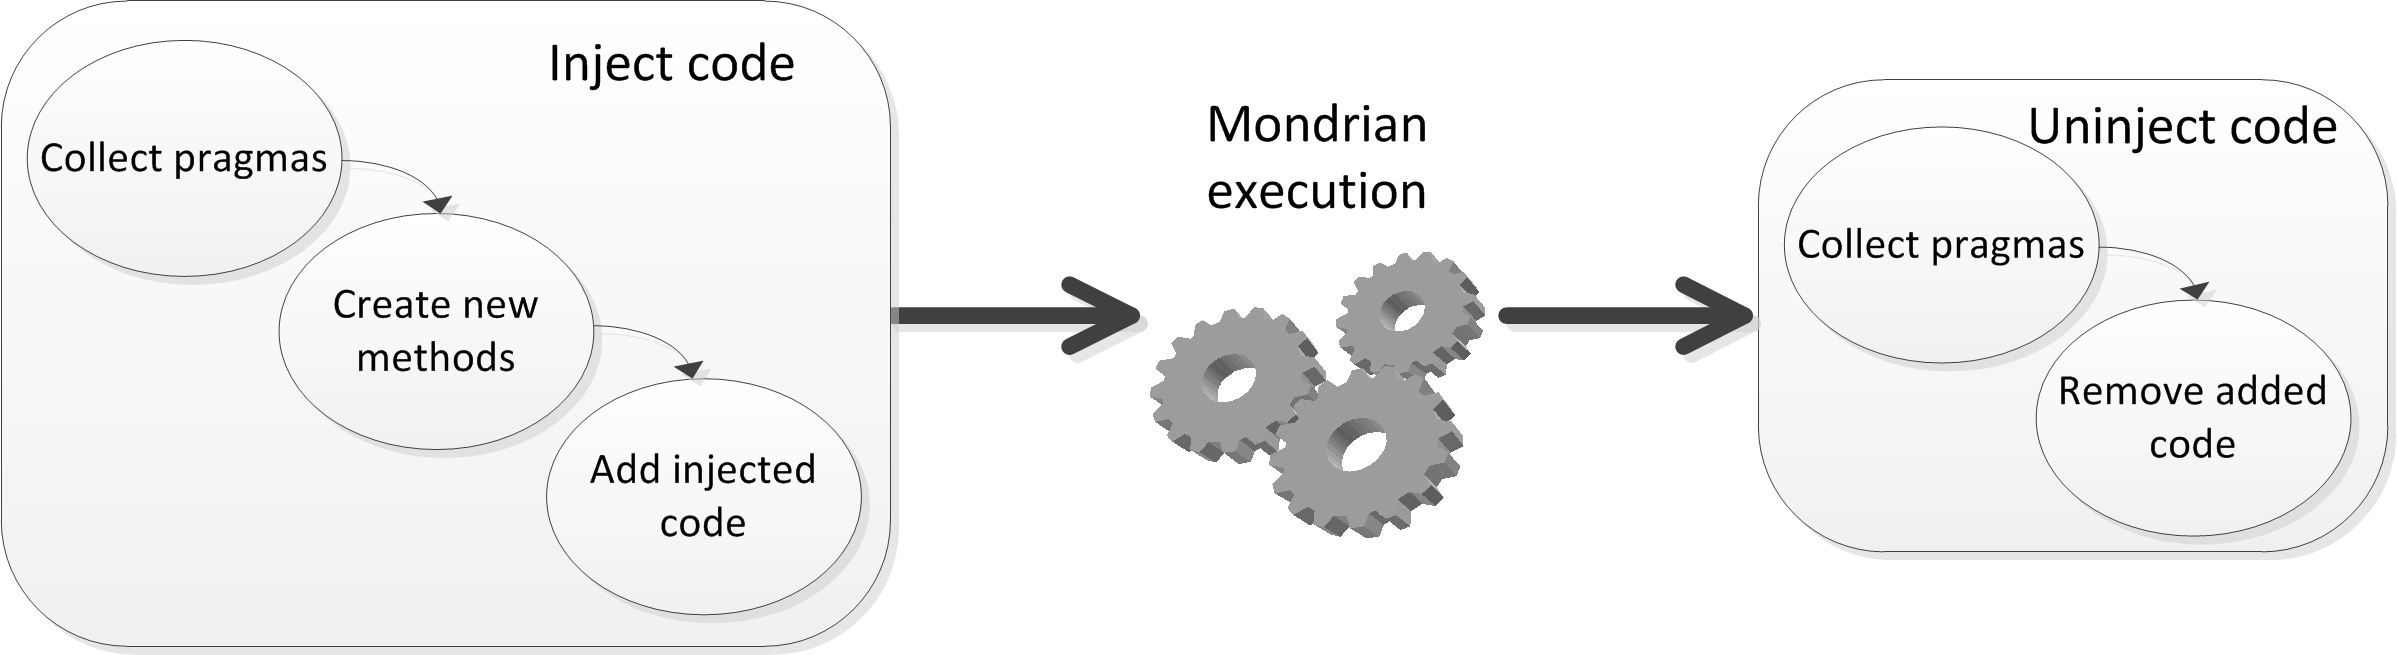
\includegraphics[scale=0.8]{InjectionMechanism} 
\par\end{centering}

\caption{Injection mechanism.\label{fig:Injection-mechanism.}}

\end{figure}


In order to automatically generate the code to be injected, the injector
code mechanism provides a \emph{CachePattern} interface. In this way,
each cache pattern has to implements this interface which allow the
generation of the methods mentioned above. Basically each subclass
is responsible of the definition of the pragma to be used and the
generation of the code sentences to be injected related with the cache
whereas the interface \emph{CachePattern} creates the methods to be
added to the system. This class hierarchy is shown in Fig. \ref{fig:Pattern-hierarchy.}.
%
\begin{figure}
\begin{centering}
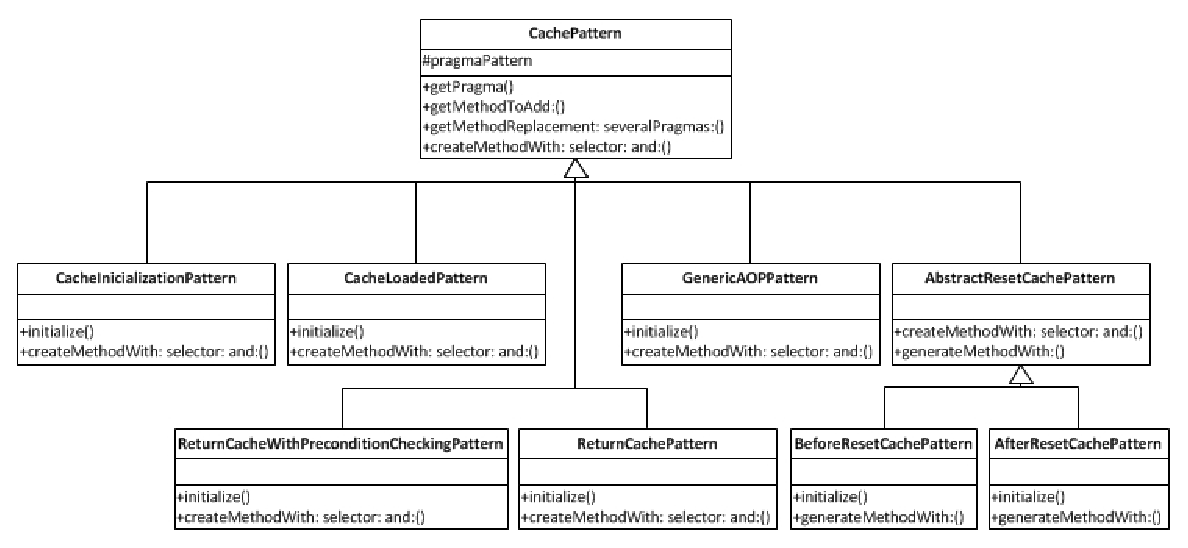
\includegraphics{PatternInheritance}
\par\end{centering}

\caption{Pattern hierarchy.\label{fig:Pattern-hierarchy.}}

\end{figure}


Next, the refactorizations applied to each code pattern are presented.

\emph{Reset Cache}: In order to refactor this pattern each statement
that resets a cache was extracted using a pragma. The pragma contains
the cache to be resetted. Owing to in some cases the resets are done
at the beginning of a method and others at the end, a hierarchy of
Reset Cache pattern is created. As is shown in Fig. \ref{fig:Pattern-hierarchy.},
this hierarchy is compose by the classes \emph{AbstractResetCachePattern},
\emph{BeforeResetCachePattern}, and \emph{AfterResetCachePattern}.
The pragmas are defined in the classes at the bottom of the hierarchy
as $<$BeforeResetCachePatternForCache: cacheName$>$ and $<$AfterResetCachePatternForCache:
cacheName$>$ respectively. For example, in the case presented in Section
\ref{sub:Pattern-Identification} of the method \emph{resetCache},
a pragma is defined for each reset of a cache leaving a cleaner code
in the method. In this case all the resets are done before the method
call, so the pragmas used are the defined by \emph{BeforeResetCachePattern}.
Even though the order of calls is changed (in comparison with the
original method), the method behavior is not modified. The code to
be generated will be reset mechanism corresponding to the cache defined
in the pragma. Following, the refactored code is presented:

\begin{lstlisting} 
MOGraphElement>>resetCache 
	<BeforeResetCachePatternForCache: #absoluteBoundsCache> 
	<BeforeResetCachePatternForCache: #elementsToDisplayCache>
	<BeforeResetCachePatternForCache: #boundsCache> 
	<BeforeResetCachePatternForCache: #cacheShapeBounds> 
	self resetElementsToLookup. 
	self resetMetricCaches
\end{lstlisting}

After the code injection the resetCache method is transformed into:

\begin{lstlisting} 
MOGraphElement>>resetCache 
	absoluteBoundsCache:=nil.
	elementsToDisplayCache:=nil. 
	boundsCache:=nil. 
	cacheShapeBounds:=SmallDictionary new. 
	self computeMOGraphElementresetCache 
\end{lstlisting}

where the method computeMOGraphElementresetCache is:

\begin{lstlisting} 
MOGraphElement>>computeMOGraphElementresetCache
	self resetElementsToLookup. 
	self resetMetricCaches 
\end{lstlisting}

This mechanism of injection of the generated code is the same for
the rest of the patterns.

\emph{Return Cache with Precondition Checking}: To refactor this pattern
the precondition checking is encapsulated into a pragma defined as
$<$ReturnCacheWithPreconditionCheckingPattern: cacheName$>$. Given that
the cache is initialized with a value when the precondition fails,
the original method is modified to return this value. For example,
in the case of the \emph{bounds} method presented in the previous
section, the code related to the cache is extracted using the pragma
and only the value to initialize the cache remains in the method as
shown the code below:

\begin{lstlisting} 
MOEdge>>bounds 
	<ReturnCacheWithPreconditionCheckingPattern: #boundsCache> 
	self shape computeBoundsFor: self. 
\end{lstlisting}

In this way, the code to be generated for this example will be \emph{boundsCache
ifNotNil: {[} \textasciicircum{} boundsCache{]}. \textasciicircum{}
boundsCache:= computeMOEdgeBounds.}

\emph{Cache Initialization}: The refactorization of this cache is
similar to the last one. Given that the structure of the pattern is
an assignation, the first section of the assignation (\emph{cacheName:=})
will be generated automatically by the code injection mechanism using
a pragma defined as $<$CacheInicializationPatternForCache: cacheName$>$.
So, only the value at which is initialized remains in the method.
In the case of the example presented in Section \ref{sub:Pattern-Identification},
the refactored code is shown below:

\begin{lstlisting} 
MOGraphElement>>cacheCanvas: aCanvas 
	<CacheInicializationPatternForCache: #cacheForm>  
	(aCanvas form copy: ((self bounds origin + aCanvas origin
	- (1@1)) extent: (self bounds extent + (2@2)))). 
\end{lstlisting}

\emph{Return Cache}: In this refactorization the entire return clause
is encapsulated by the pragma. The pragma is defined as $<$ReturnCacheWithPreconditionCheckingPattern:
cacheName$>$. Following, the refactored code for the example shown in
the last section is presented:

\begin{lstlisting}
 MOGraphElement>>shapeBounds 
	<ReturnCachePatternForCache: #cacheShapeBounds> 
\end{lstlisting}

\emph{Cache Loaded:} In order to refactor this pattern the cache checking
is encapsulated by a pragma defined as $<$CacheLoadedPatternForCache:
cacheName$>$. The code generated contains a sentence in which the checking
is done for all the caches defined in the pragmas of this pattern
contained in a method. In the case of the example presented in Section
\ref{sub:Pattern-Identification}, the refactored code is shown below:
\begin{lstlisting} 
MOGraphElement>>isCacheLoaded 
	<CacheLoadedPatternForCache: #cacheForm>
\end{lstlisting}

With the use of these patterns the \emph{Cache Concern} is refactorized
properly in more than 85\% of the methods of the MOGraphElement hierarchy.
All the other uses of the caches (those that are not encapsulated
by patterns) are also refactored by means of pragmas. For these cases
a \emph{Generic AOP} pattern is used. The pragmas used have the structure
\emph{$<$cache: cacheName before: '' after: ''$>$} where \emph{cache}
indicates the name of the cache that will be injected. The clauses
before and after indicate the source code that will be injected and
when it will be injected in regard to the execution of the method.
That is to say, the code inside the original method will be replaced
by the code pointed out in the before clause of the pragma, a call
to the new method will be added, and the code contained in the after
clause of the pragma will be added at the end.

The use of the presented patterns could be used to compose the caches
behavior improving the maintenance of the system. In this line, the
contribution of the approach is twofold. First, the mechanism of encapsulation
and injection could be used to refactor the currently Mondrian caches
(and also those that may be introduced in future) improving the code
reuse. Second, the code legibility is increased because the \emph{Cache
Concern} is extracted from the main concern leaving a cleaner code.

The cache composition is achieved during the injection phase. As the
different pieces of code that are related to the cache are encapsulated
by means of the patterns, an implicit process of division of the complexity
of the caches behavior is achieved. That is to say, this kind of approach
helps the developer by splitting the caches behavior is smalls fragments
of code. These fragments of code are encapsulated by the patterns
and they are finally composed during the injection phase. For example,
the functionality related to the cache \emph{absoluteBoundsCache}
is refactored by the patterns \emph{Reset Cache,} \emph{Return Cache
with Precondition Checking,} and \emph{Cache Initialization}.

% % % % % % % % % % % % % % % % % % % % % % % % % % % % % % % % % %
\section{Benefits}\seclabel{benefits}

\ab{What are the benefits of the approach? Can I unplug cache?}

% % % % % % % % % % % % % % % % % % % % % % % % % % % % % % % % % %
\section{Conclusion}\seclabel{conclusion}



% % % % % % % % % % % % % % % % % % % % % % % % % % % % % % % % % %
\section*{Acknowledgments}

\small We gratefully thanks ...

% bibliography
% % % % % % % % % % % % % % % % % % % % % % % % % % % % % % % % %
\bibliographystyle{splncs}
\bibliography{scg}

\end{document}

% % % % % % % % % % % % % % % % % % % % % % % % % % % % % % % % % %
% % % % % % % % % % % % % % % % % % % % % % % % % % % % % % % % % %
% % % % % % % % % % % % % % % % % % % % % % % % % % % % % % % % % %
% % % % % % % % % % % % % % % % % % % % % % % % % % % % % % % % % %
% % % % % % % % % % % % % % % % % % % % % % % % % % % % % % % % % %
% % % % % % % % % % % % % % % % % % % % % % % % % % % % % % % % % %
% % % % % % % % % % % % % % % % % % % % % % % % % % % % % % % % % %
% % % % % % % % % % % % % % % % % % % % % % % % % % % % % % % % % %

\begin{lstlisting} 
MOGraphElement>>cacheCanvas: aCanvas 
	<cache: #cacheForm before: 'cacheForm :=' after: ''> 
	^(aCanvas form copy: ((self bounds origin + aCanvas origin - (1@1)) 
	extent: (self bounds extent + (2@2)))). 
\end{lstlisting}

\emph{Return Cache}: In this refactorization the entire return clause
is encapsulated into the pragma. The after clause is used to contain
the code because some computations can be performed before returning
the cache. Following, the refactored code for the example presented
in the last section is presented:

\begin{lstlisting} 
MOGraphElement>>shapeBounds 
	<cache: #cacheShapeBounds before: '' after: '.^ cacheShapeBounds.'> 
\end{lstlisting}

\paragraph{What we would like to have}\ \\
The programmer, instead of writting:
\begin{lstlisting}
MOGraphElement>>absoluteBounds
	absoluteBoundsCache ifNotNil: [ ^ absoluteBoundsCache ].
	^ absoluteBoundsCache := self shape absoluteBoundsFor: self
\end{lstlisting}

He/She should write:

\begin{lstlisting}
MOGraphElement>>absoluteBounds
	<cache: #absoluteBoundsCache>
	 ^ self shape absoluteBoundsFor: self
\end{lstlisting}

Then, our cache injector mechanism will produce the code:
\begin{lstlisting}
MOGraphElement>>absoluteBounds
	<instrumented>
	<cache: #absoluteBoundsCache>
	absoluteBoundsCache ifNotNil: [ ^ absoluteBoundsCache ].
	 ^ absoluteBoundsCache  := self  computeAbsoluteBounds.
	
MOGraphElement>> computeAbsoluteBounds
	^ self shape absoluteBoundsFor: self
\end{lstlisting}



\paragraph{What we have now in our implementation}

The code
\begin{lstlisting}
MOGraphElement>>absoluteBounds
	"Answer the bounds in absolute terms (relative to the entire Canvas, not just the parent)."
	absoluteBoundsCache ifNotNil: [ ^ absoluteBoundsCache ].
	^ absoluteBoundsCache := self shape absoluteBoundsFor: self
\end{lstlisting}

is transformed into 

\begin{lstlisting}
MOGraphElement>>absoluteBounds
<cache: #absoluteBoundsCache before: 'absoluteBoundsCache ifNotNil: [ ^ absoluteBoundsCache ]. ^ absoluteBoundsCache := (' after: ' )'>
	"Answer the bounds in absolute terms (relative to the entire Canvas, not just the parent)."
	 ^ self shape absoluteBoundsFor: self
\end{lstlisting}

\begin{lstlisting}
bounds
	"Answer the bounds of the receiver."
	"the bounds is has an absolute origin"
	"Note that the bounds computed above, may have (and it is likely to) a different origin. The reason is that the layout is in charge to position the nodes properly"
	| basicBounds |

	boundsCache ifNotNil: [ ^ boundsCache ].

	"We check if  the shape if present"
	self shapeBoundsAt: self shape ifPresent: [ :b | ^ boundsCache := b ].

	basicBounds := self shape computeBoundsFor: self.
	self shapeBoundsAt: self shape put: basicBounds.
	^ boundsCache := basicBounds
\end{lstlisting}

is refactorized into:

\begin{lstlisting}
bounds
<cache: #boundsCache before: 'boundsCache ifNotNil: [ ^ boundsCache ]. self shapeBoundsAt: self shape ifPresent: [ :b | ^ boundsCache := b ]. ^ boundsCache :=' after: ''>
	"Answer the bounds of the receiver."
	"the bounds is has an absolute origin"
	"Note that the bounds computed above, may have (and it is likely to) a different origin. The reason is that the layout is in charge to position the nodes properly"
	| basicBounds |
	basicBounds := self shape computeBoundsFor: self.
	self shapeBoundsAt: self shape put: basicBounds.
	^ basicBounds
\end{lstlisting}

\begin{lstlisting}
cacheCanvas: aCanvas
	cacheForm := aCanvas form copy: ((self bounds origin + aCanvas origin - (1@1)) 
													extent: (self bounds extent + (2@2))).
\end{lstlisting}

is transformed into:

\begin{lstlisting}
cacheCanvas: aCanvas
<cache: #cacheForm before: 'cacheForm :=' after: ''>
	^(aCanvas form copy: ((self bounds origin + aCanvas origin - (1@1)) 
													extent: (self bounds extent + (2@2)))).
\end{lstlisting}


\begin{lstlisting}
elementsToDisplay

	elementsToDisplayCache ifNotNil: [ ^ elementsToDisplayCache ].
	^ elementsToDisplayCache := self computeElementsToDisplay
\end{lstlisting}

is transformed into:

\begin{lstlisting}
elementsToDisplay
<cache: #elementsToDisplayCache before: 'elementsToDisplayCache ifNotNil: [ ^ elementsToDisplayCache ]. ^ elementsToDisplayCache := (' after: ' )'>
^ self compute2ElementsToDisplay
\end{lstlisting}	

\begin{lstlisting}
hasCachedForm
	^ cacheForm notNil
\end{lstlisting}	

transformed into:

\begin{lstlisting}
hasCachedForm
<cache: #cacheForm before: '' after: '.^ cacheForm notNil.'>
\end{lstlisting}	

\begin{lstlisting}
nodeWith: anObject ifAbsent: aBlock 
	| nodeLookedUp |
	lookupNodeCache ifNil: [ lookupNodeCache := IdentityDictionary new ].
	lookupNodeCache at: anObject ifPresent: [ :v | ^ v ].
	nodeLookedUp := self nodes detect: [:each | each model = anObject ] ifNone: aBlock.
	lookupNodeCache at: anObject put: nodeLookedUp.
	^ nodeLookedUp
\end{lstlisting}

\begin{lstlisting}
nodeWith: anObject ifAbsent: aBlock 
<cache: #lookupNodeCache before:'	lookupNodeCache ifNil: [ lookupNodeCache := IdentityDictionary new ]. lookupNodeCache at: anObject ifPresent: [ :v | ^ v ]. ^lookupNodeCache at: anObject put: (' after: ' )'>
	^ self nodes detect: [:each | each model = anObject ] ifNone: aBlock.
\end{lstlisting}


\begin{lstlisting}
resetCache
	self resetElementsToLookup.
	boundsCache := absoluteBoundsCache := nil.	"Having IdentityDictionary instead of SmallDictionary works the same, it is faster although"
	cacheShapeBounds := SmallDictionary new.	"cacheShapeBounds := IdentityDictionary new"
	elementsToDisplayCache := nil.
	self resetMetricCaches
\end{lstlisting}
transformed into:
\begin{lstlisting}
resetCache
<cache: #absoluteBoundsCache before: 'absoluteBoundsCache := nil.' after: ''> 
<cache: #elementsToDisplayCache before: 'elementsToDisplayCache := nil.' after: ''> 
<cache:#boundsCache before: 'boundsCache:= nil.' after: ''> 
<cache: #cacheShapeBounds before: 'cacheShapeBounds := SmallDictionary new.' after: ''>

	self resetElementsToLookup.
	self resetMetricCaches
\end{lstlisting}

\begin{lstlisting}
MONode>>displayOn: aCanvas 
	"	self layer isVisible ifFalse: [ ^ self ]."	
	| b canvas |
	(aCanvas isVisible: self absoluteBounds) ifFalse: [ ^ self ].

	self isCacheLoaded ifTrue: [
		aCanvas paintImage: cacheForm at: (self absoluteBounds origin - (1@1)).
		^ self ].
	
	self shouldCache ifFalse: [ 
		"If we cannot cache (for example if we are too big) then we display ourself, and iterate over inner nodes
		 while giving them a chance to cache"
		self displayWithoutCachingOn: aCanvas.
		^ self ].	
	
	b := self bounds.	
	canvas := FormCanvas extent: (b extent + (2@2)) .

	canvas 
		translateBy: self absoluteBounds origin negated + (1@1) 
		during: [:tmpCanvas | self displayWithoutCachingOn: tmpCanvas ].
	cacheForm := canvas form.	

	self updateOwner. 
	aCanvas paintImage: cacheForm at: (self absoluteBounds origin - (1@1)).
\end{lstlisting}

\begin{lstlisting}
MONode>>displayOn: aCanvas 
<cache: #cacheForm before: '(aCanvas isVisible: self absoluteBounds) ifFalse: [ ^ self ]. self isCacheLoaded ifTrue: [
		aCanvas paintImage: cacheForm at: (self absoluteBounds origin - (1@1)).
		^ self ]. self shouldCache ifFalse: [ self displayWithoutCachingOn: aCanvas. ^ self ]. cacheForm := ' after: '.self updateOwner. 
	aCanvas paintImage: cacheForm at: (self absoluteBounds origin - (1@1)).'>

	| b canvas |
	b := self bounds.	
	canvas := FormCanvas extent: (b extent + (2@2)) .
		
	canvas 
		translateBy: self absoluteBounds origin negated + (1@1) 
		during: [:tmpCanvas | self displayWithoutCachingOn: tmpCanvas ].
	^ canvas form.	
\end{lstlisting}

\begin{lstlisting}
translateBy: aPoint bounded: bounded
	"It moves the element by aPoint. 
	If bounded is true and the owner is not the root, 
	then the bounds are limited by the owner bounds.
	If the element is placed in the root, then the root's bounds are updated"
	| realStep newRelativePosition allShapes |
	self shapeBounds isNil ifTrue: [ ^ self bounds ].
	self shapeBounds isEmpty ifTrue: [ ^ self bounds ].

	realStep :=  bounded 
						ifTrue: [ self getBoundedTranslationStep: aPoint ]
						ifFalse: [ aPoint ].			

	newRelativePosition := self origin + aPoint.	

	allShapes := self shapeBounds keys.
	allShapes do: [ :eachShape | 
		self shapeBoundsAt: eachShape put: ((self shapeBoundsAt: eachShape) translateBy: realStep) ].
	boundsCache := absoluteBoundsCache := nil.
	self allNodesDo: [ :n | n translateAbsoluteCacheBy: realStep ].

	
	owner isRoot ifTrue: [
		"the root has to be extended in any case"
		owner expandToIncludePoint: (newRelativePosition +  self bounds extent) ].
	
	self resetCacheInEdges
\end{lstlisting}

\begin{lstlisting}
translateBy: aPoint bounded: bounded
<cache: #boundsCache before: '' after: '.boundsCache :=nil.'>
<cache: #absoluteBoundsCache before: '' after: 'absoluteBoundsCache := nil.'>
	"It moves the element by aPoint. 
	If bounded is true and the owner is not the root, 
	then the bounds are limited by the owner bounds.
	If the element is placed in the root, then the root's bounds are updated"
	| realStep newRelativePosition allShapes |
	self shapeBounds isNil ifTrue: [ ^ self bounds ].
	self shapeBounds isEmpty ifTrue: [ ^ self bounds ].

	realStep :=  bounded 
						ifTrue: [ self getBoundedTranslationStep: aPoint ]
						ifFalse: [ aPoint ].			

	newRelativePosition := self origin + aPoint.	

	allShapes := self shapeBounds keys.
	allShapes do: [ :eachShape | 
		self shapeBoundsAt: eachShape put: ((self shapeBoundsAt: eachShape) translateBy: realStep) ].
	
	owner isRoot ifTrue: [
		"the root has to be extended in any case"
		owner expandToIncludePoint: (newRelativePosition +  self bounds extent) ].
	
	
	"boundsCache := absoluteBoundsCache := nil."
	self allNodesDo: [ :n | n translateAbsoluteCacheBy: realStep ].
	self resetCacheInEdges
\end{lstlisting}

\begin{lstlisting}
NONode>>bounds
	^ boundsCache ifNil: [ boundsCache := self shape computeBoundsFor: self ].
\end{lstlisting}

\begin{lstlisting}
NONode>>bounds
<cache: #boundsCache before: '^ boundsCache ifNil: [boundsCache :=' after: ' ]'>
	^self shape computeBoundsFor: self.
\end{lstlisting}
